% Chapter 1

\chapter{Introducción general} % Main chapter title

\label{Chapter1} % For referencing the chapter elsewhere, use \ref{Chapter1} 
\label{IntroGeneral}

%----------------------------------------------------------------------------------------

% Define some commands to keep the formatting separated from the content 
\newcommand{\keyword}[1]{\textbf{#1}}
\newcommand{\tabhead}[1]{\textbf{#1}}
\newcommand{\code}[1]{\texttt{#1}}
\newcommand{\file}[1]{\texttt{\bfseries#1}}
\newcommand{\option}[1]{\texttt{\itshape#1}}
\newcommand{\grados}{$^{\circ}$}

En este capítulo se presenta una introducción a los transformadores y sus ensayos de caracterización más comunes. Asimismo, se introducen algunos equipos disponibles en el mercado y por último, se aborda el alcance y objetivo del trabajo realizado.

%----------------------------------------------------------------------------------------

%\section{Introducción}

%----------------------------------------------------------------------------------------
\section{Introducción a los transformadores}

Un transformador eléctrico es una máquina estática de corriente alterna que permite aumentar o disminuir la tensión y corriente de un circuito. La frecuencia de la onda de entrada se mantiene invariable a la salida y, en el caso de un transformador ideal, la potencia también se mantiene constante. El transformador utiliza el principio de la inducción electromagnética para su funcionamiento. En la figura \ref{fig:figTransformador} se muestra la imagen de un transformador típico de baja tensión \citep{TRAFO_WIKI}, \citep{TRAFO_2}.

\begin{figure}[h]
	\centering
	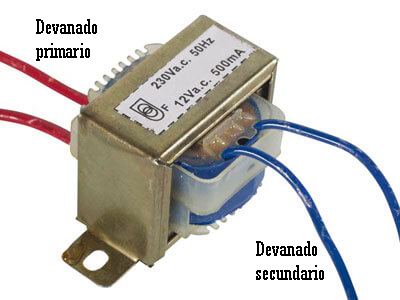
\includegraphics[scale=.5]{./Figures/transformador.jpg}
	\caption{Transformador de baja potencia\protect\footnotemark.}
	\label{fig:figTransformador}
\end{figure}

\footnotetext{Imagen tomada de \url{https://www.ingmecafenix.com/electronica/transformador-electrico/}}

El transformador está constituido por dos bobinas de material conductor devanadas sobre un núcleo cerrado de material ferromagnético. Los bobinados se denominan primario y secundario según corresponda a la entrada o salida del sistema, respectivamente. Las bobinas o bobinados están aislados eléctricamente entre sí, la única conexión entre estos la constituye el flujo magnético que se establece en el núcleo por la circulación de corriente por dichos bobinados. Por su parte, el núcleo generalmente se fabrica de láminas apiladas de hierro o acero, de esta forma, se optimiza el flujo magnético generado por las corrientes circulantes en los bobinados. En la figura \ref{fig:figTransformador2} se muestra el principio de funcionamiento de un transformador.

\begin{figure}[htpb]
	\centering
	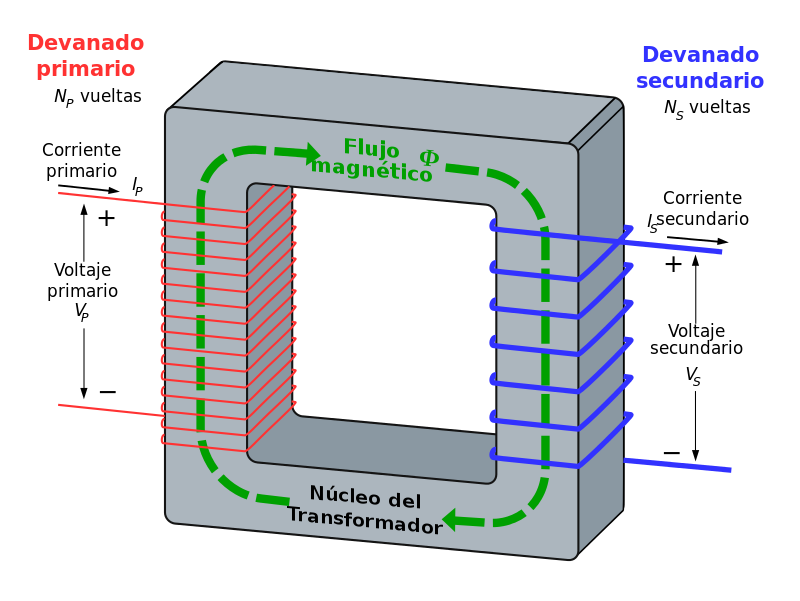
\includegraphics[scale=.3]{./Figures/transformador_2.png}
	\caption{Transformador monofásico ideal\protect\footnotemark.}
	\label{fig:figTransformador2}
\end{figure}

\footnotetext{Imagen tomada de \url{https://es.wikipedia.org/wiki/Transformador}}

Existen transformadores con más de dos bobinados y diferentes arquitecturas de conexionado, un ejemplo lo constituye el transformador trifásico que está formado por 6 bobinados que pueden ser conectados en estrella o triangulo.

Actualmente, se pueden encontrar una gran variedad de transformadores para infinidad de aplicaciones. Una clasificación posible es la siguiente \citep{TRAFO_APL}:

\begin{itemize}
\item Transformador de potencia.
\item Transformador de distribución.
\item Autotransformador.
\item Transformador de corriente.
\item Transformador de potencial.
\end{itemize}

Las aplicaciones van desde cargadores de teléfonos móviles hasta transformadores de potencia para estaciones y subestaciones de energía eléctrica.

\subsection{Caracterización de transformadores}

Para los cálculos de circuitos o líneas con transformadores se utiliza un circuito equivalente que representa el comportamiento del transformador real. Para la mayoría de los casos es suficiente con que dicho circuito equivalente represente el transformador en régimen permanente \citep{TRAFO_WIKI}. 

En general, se deben desarrollar diferentes ensayos sobre el transformador para determinar los parámetros de un circuito equivalente, entre los ensayos más comunes tenemos:

\begin{itemize}
\item Ensayo de vacío.
\item Ensayo de cortocircuito.
\item Ensayo de aislamiento.
\end{itemize}

En las siguientes secciones se brinda una introducción a los ensayos mencionados.

\subsubsection{Ensayo de vacío}

El ensayo de vacío es un método utilizado para determinar diversos parámetros del transformador mediante pruebas realizadas sin aplicar carga \citep{TRAFO_VACIO}. En la figura \ref{fig:figEnsayoVacio} se muestra el conexionado para este ensayo.

En este ensayo se alimenta el bobinado primario con la tensión nominal, se deja el secundario sin carga y se debe medir la tensión en los bornes del primario, la tensión en los bornes del secundario, la corriente en el devanado primario y la potencia del primario. 

\begin{figure}[htpb]
	\centering
	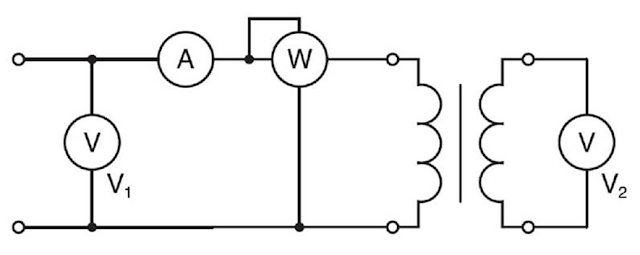
\includegraphics[scale=.4]{./Figures/EnsayoVacio.png}
	\caption{Ensayo de vacío.}
	\label{fig:figEnsayoVacio}
\end{figure}

\subsubsection{Ensayo de cortocircuito}
El ensayo de cortocircuito permite determinar la impedancia de cortocircuito o impedancia en serie del transformador \citep{TRAFO_CORTO}. La impedancia de cortocircuito representa las pérdidas en el cobre de los devanados, así como la inductancia de dispersión y otras inductancias parásitas. En la figura \ref{fig:figEnsayoCorto} se muestra el conexionado para este ensayo.

\begin{figure}[htpb]
	\centering
	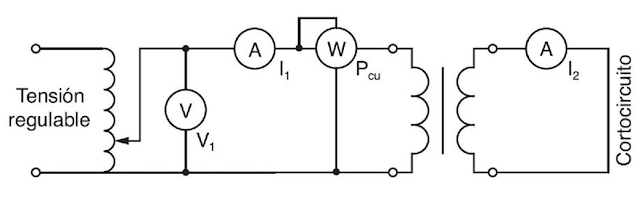
\includegraphics[scale=.5]{./Figures/EnsayoCorto.png}
	\caption{Ensayo de cortocircuito.}
	\label{fig:figEnsayoCorto}
\end{figure}

En este ensayo se alimenta el bobinado primario con una tensión muy reducida, se coloca un cortocircuito en el bobinado secundario y se debe medir la tensión resultante en los bornes del primario, la corriente en el bobinado secundario, la corriente en el devanado primario y la potencia del primario. Para conseguir los valores reducidos de tensión es necesario un sistema de tensión ajustable como puede ser un autotransformador regulable. La tensión aplicada en el primario debe ser tal que haga circular la corriente nominal por el bobinado secundario.

\subsubsection{Ensayo de aislamiento}

El ensayo de aislamiento permite determinar el estado del dieléctrico o aislante entre fases o entre una fase y el chasis del transformador \citep{TRAFO_AISL}. La medida suele dar valores en el orden de los megaohmios, valor que se ve reducido si el aislante está deteriorado.

En la figura \ref{fig:figEnsayoAislacion} se muestra un ensayo de aislamiento entre bobinas.

\begin{figure}[htpb]
	\centering
	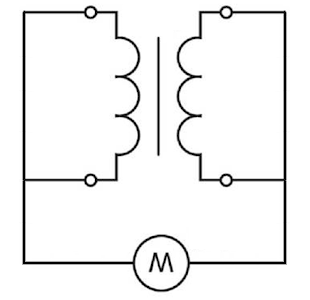
\includegraphics[scale=.5]{./Figures/EnsayoAislacion.png}
	\caption{Ensayo de aislamiento entre bobinas.}
	\label{fig:figEnsayoAislacion}
\end{figure}


%----------------------------------------------------------------------------------------

\section{Estado del arte}
En la actualidad existe una variedad de equipos con el fin de caracterizar transformadores de baja tensión. Estos son capaces de caracterizar transformadores de tensión y corriente, sobre los cuales se pueden realizar múltiples ensayos y así determinar diferentes parámetros. A su vez, cuentan con interfaces de comunicación variadas como Wi-Fi, Ethernet y USB, por medio de las cuales se pueden descargar los datos medidos a una computadora para su posterior análisis. Un punto importante de estos equipos es que por lo general poseen certificaciones internaciones como por ejemplo IECs para los procedimientos de medición.

Como ejemplos podemos citar el modelo MVCT de Megger \citep{MVCT} y el modelo iCT1 de Alta Nova \citep{iCT1}. En la tabla \ref{tab:EstArte} se muestra una comparativa entre ambos equipos.

\begin{table}[htpb]
\centering
\caption[Estado del arte]{Comparación de equipos comerciales.}
\resizebox{\textwidth}{!}{%
\begin{tabular}{c c c}
\hline
\toprule
\textbf{Características/Ensayos}                           & \begin{tabular}[c]{@{}c@{}}\textbf{MVCT} \\\textbf{(Megger)} \end{tabular}& \begin{tabular}[c]{@{}c@{}}\textbf{ICT1} \\\textbf{(Alta Nova)} \end{tabular}\\ \hline
Apto para transformador de corriente (TI) y tensión (TC)   & x                      & x                \\
Ensayo de relación de transformación                       & x                      & x                \\
Resistencia de bobinados                                   & x                      & x                \\
Desviación de fase                                         & x                      & x                \\
Curva de saturación (TI)                                   & x                      & x                \\
Desmagnetización (TI)                                      & x                      & x                \\
Aislamiento                                                & x                      & x                \\
Interfaz Ethernet                                          & x                      & x                \\
Interfaz Wi-Fi                                             &                        & x                \\
Interfaz USB                                               & x                      & x                \\
\bottomrule
\hline
\end{tabular}%
}
\label{tab:EstArte}
\end{table}

%----------------------------------------------------------------------------------------

\section{Motivación}
Los transformadores son una parte esencial en muchos campos de la industria, son parte fundamental en el sistema de distribución de energía, así como en equipos que son alimentados desde la red. Por esta razón, es de vital importancia su estudio y establecer métodos para conocer su estado antes de su instalación y durante su servicio.

El transformador debe estar en óptimas condiciones al momento de su instalación para evitar posibles fallas del sistema donde es instalado. Un transformador cuyos parámetros esenciales están fuera de especificación puede generar un mal funcionamiento o inclusive sacar de servicio al sistema. Como ejemplo podemos citar los sistemas de distribución de energía eléctrica ya que deben ser sistemas de muy alta disponibilidad, donde un fallo en los componentes de estos sistemas puede devenir en la caída parcial o total del sistema distribución.

En el caso particular de la empresa Iris Tecnología S.R.L., que fabrica equipos electromédicos, necesita conocer si los transformadores provistos son aptos para ser utilizados en sus equipos. Para ello, la empresa cuenta con un sistema de calidad basado en la norma ISO13485:2016.

Entre las tareas y controles necesarios para el sistema de calidad se encuentra el ensayo y calificación de transformadores. Actualmente, esta tarea es realizada manualmente por un operador. Esta labor, además de insumir una gran cantidad de tiempo y ser muy repetitiva, presenta un gran riesgo de error humano y puede comprometer la seguridad del operario y la fiabilidad de los datos obtenidos.

La posibilidad de contar con un equipamiento que, con una mínima intervención del operador, pueda desarrollar los ensayos requeridos representa una gran ventaja para la empresa.

%----------------------------------------------------------------------------------------

\section{Objetivos y alcance}

\subsection{Objetivos del trabajo}

El objetivo de este trabajo fue el desarrollo de un prototipo de hardware y software que permite automatizar el proceso de caracterización de transformadores de baja tensión utilizado. El prototipo desarrollado es casi autónomo, es decir, solo requiere una mínima intervención del operador para funcionar. Por otro lado, los resultados de la caracterización son enviados a un servidor web proporcionado por el cliente, mostrados en un \textit{display} local e impresos en una etiqueta.

\subsection{Alcance del trabajo}
El presente trabajo tiene como alcance:
\begin{itemize}
\item El análisis, investigación y elección del hardware.
\item La investigación del modelo de impresora a adquirir, cuyo protocolo debe estar disponible.
\item El diseño e implementación del firmware del sistema en lenguaje C sobre FreeRTOS.
\item El desarrollo de un prototipo funcional sobre un circuito impreso universal.
\end{itemize}

Queda excluido del alcance de este trabajo:
\begin{itemize}
\item El desarrollo de circuitos de medición de tensión y/o corriente alterna de precisión. Se acepta la precisión obtenida de módulos comerciales como el ZMPT101B.
\item El desarrollo de fuentes de tensión alterna de precisión para alimentar los transformadores en ensayo.
\item El desarrollo de una aplicación web desde la cual interactuar por Wi-Fi con el módulo.
\item El desarrollo del servidor web o API de colección de datos.
\item El desarrollo de un prototipo de fabricación escalable que cumpla con todas las certificaciones necesarias.
\item El desarrollo de un circuito impreso, más allá del prototipo en placa universal.
\item El diseño de circuitos de protección del operario contra descargas eléctricas de alta tensión. En este sentido, se asume que el operario que utilizará el dispositivo es idóneo en el tema. Asimismo, se asume que el cliente posee en sus instalaciones las medidas de seguridad pertinentes para el trabajo con altas tensiones, como disyuntores y puestas a tierras, acorde con la normativa vigente de Higiene y Seguridad en el Trabajo.
\end{itemize}
